\chapter{Introduction}
\label{chap:introduction}

To help readers get better acquainted with the topic, introduction is divided into four sections. First section covers general motivation and relevance of the project. Next section describes state of technology, market and consumer trends at the time this thesis was published. The following section lays out project goals and defines the scope they will be tackled on while in the last section, project structure is outlined so that readers can easily navigate through this thesis body.


\section{Motivation}

Sleep is seemingly a trivial thing - from the moment that they are born, all humans have a need to sleep. It is a natural function in the same way breathing and other vital body functions are. Having slept for adequate time and with good quality tends to make people feel good and have more energy performing their daily tasks. When a person did not sleep well or did not sleep enough it will usually negatively reflect both on their body and their behaviour. National Sleep Foundation along with multi-disciplinary expert panel recommends sleep time for each age group ranging from 14 to 17 hours daily for newborns to between 7 and 8 hours for older adults\cite{NSF}. Sleep deprivation effects motor and cognitive abilities as well as mood but these effects can also occur in cases of bad sleep quality regardless of the sleep duration\cite{doi:10.1093/sleep/19.4.318}. That same sleep quality is influenced by many factors ranging from physical ones such as sleeping environment and position to subjective ones such as emotional state and dreams. As clear separation of these factors is rarely possible, most of the researches relied on the isolation of influences comparing results between large control and influenced groups. Sleep quality is then usually determined by questionnaires and data analysis which result in quantitative results such as Pittsburgh Sleep Quality Index\cite{psqi}.\\

To accurately and consistently determine sleep quality, sleep is divided into 4 stages. First stage is called N1 and is a transition between awakeness and sleep. Person is still conscious and aware of surroundings. Duration of this stage is usually between 5 and 10 minutes. The second stage is called N2 and is categorized by a steady breathing and hearth rate as well as with a drop in body temperature. This stage occurs multiple times during sleep and totals for around 50\% of the time spent sleeping. Together these categories can be classified as light sleep. Stages N3 and N4 can be categorized as a deep sleep as it becomes harder to wake up a person from these stages. They can be recognized by further temperature drop, lower blood pressure and by delta waves\footnote{High amplitude brain waves with a frequency of oscillation between 0.5 and 4 Hz.} emitted by the brain. Sleep state can also be categorized as \ac{NREM} or \ac{REM}. REM phase usually occurs only after an initial stage of deep sleep. It is a phase in which dreams occur whilst eyes move quickly in different directions with hearth and breathing rate becoming irregular. To prevent a person from waking up, muscles and senses below the neck become inactive. \ac{REM} phases alternate with light and deep sleep stages and tend to become longer with each alternation. Adults with a healthy sleep habits spend 20\% of time asleep in a \ac{REM} phase while this percentage becomes lower with age. Typical alternation of sleep stages during sleep is shown in \ref{fig:sleep-phases}. \\

\begin{figure}[h]
  \begin{center}
    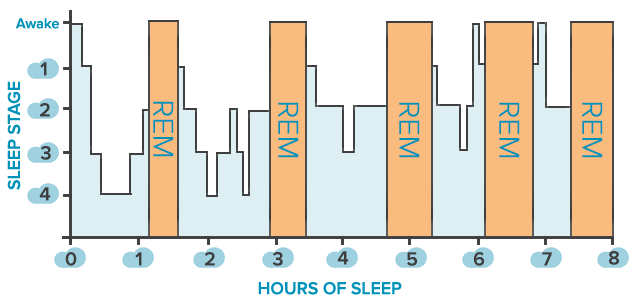
\includegraphics[width=0.7\linewidth]{0-sleep_phases.png}
  \end{center}
  \caption{Sleep phases during typical 8 hour sleep.}
  \label{fig:sleep-phases}
\end{figure}

As it is impossible to track these sleep phases personally, a variety of measurement devices is used in a study called \ac{PPG}. This study involves continuous or periodical measurement of physical parameters. Electrophysiological measurements are done with the help of \ac{EEG}, \ac{EMG} and \ac{EOG}. Drawback of using these methods is requirement of complex equipment, knowledge to evaluate the results and controlled environment which is why these measurements are usually done only for clinical or research purposes. But simple sleep monitoring can be done using much simpler processes - with heart rate, body movement and position tracking. Unlike before mentioned method these measurements can be done unobtrusively and in home environment. Improving the process and accuracy of these methods and improving correlation of collected results to the real sleep parameters may lead to much easier diagnosis of sleep disorders. Furthermore, availability and accessibility of this technology will encourage larger number of people to monitor their sleep performance which may lead to better mood, efficiency of executing daily tasks and sport results. This thesis will primarily focus on proposing a non-obtrusive way to track both sleep time and quality with a proposal of technology and measuring methods.


\section{Technology and current consumer market trends}

In the recent years, the market for sleep and fitness tracking devices has been expanding with the support of almost all major smartphone manufacturers. Some new brands specializing in the making of such devices have also emerged and have been steadily gaining the market share. Most of the devices that are currently used for consumer sleep tracking are actually multifunctional devices such as smart watches, armbands and rings. Beside sleep, they usually track physical activity, pulse and show time or provide some other information. Smart watches are additionally customizable as they usually allow for installation of third-party\footnote{Not provided by the original manufacturer} applications. This versatility makes such devices very attractive to the customer regardless of sleep tracking and monitoring quality built into the devices. To paint a better picture, in 2014 Dr. C. Winter compared a few of the most popular sleep tracking armbands to the polysomnogram\cite{Winter}. His results are showing that most of the devices, regardless of their cost, were able to distinguish between awakeness and sleep which allowed them to measure the time spent sleeping. Unfortunately, they were not able to separate REM, N1, N2 and N3 sleep phases or estimate the time spent dreaming. Some devices provided estimate if a person was in a deep or light sleep but the results were mostly inaccurate. In late 2016 J. Yoon tested newer iteration of the consumer devices and the results(\ref{fig:yoon}) show improvement of the deep or light sleep phase detection but devices are still not accurate enough to guess the real sleep phase with an acceptable degree of certainty\cite{Yoon}.


\begin{figure}[h]
  \begin{center}
    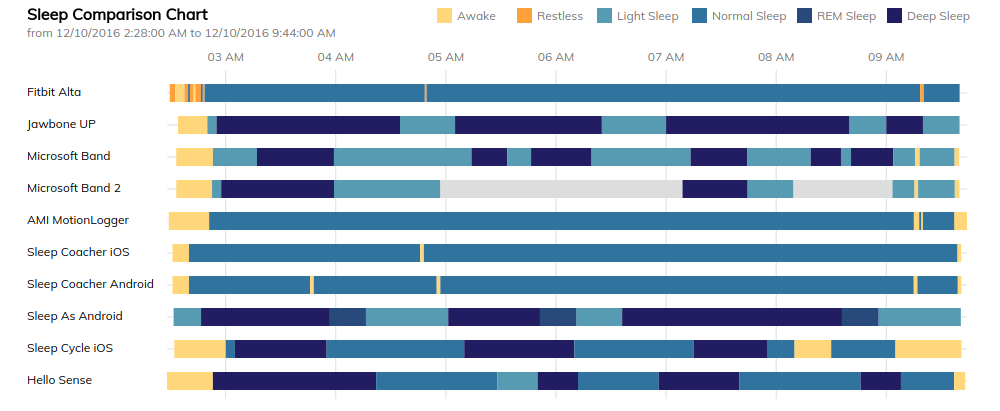
\includegraphics[width=0.8\linewidth]{0-yoon.png}
  \end{center}
  \caption{Sleep detection comparison between consumer devices}
  \label{fig:yoon}
\end{figure}

The reason for inaccuracy of consumer on-body sleep tracking devices is the underlying technology. \ac{MEMS} sensors are used for movement tracking for actigraphy\footnote{a non-invasive method of monitoring rest and activity cycles where a device worn by subject records movements} and simple photo sensors are used for \ac{PPG} which gives an estimate of pulse frequency. Most of the devices are designed in such a way that they are non-obtrusive, small, easy to use and nice looking. This means that batteries powering sleep monitoring devices must be small and device usage should be minimized to maximize the battery life. This is achieved through the use of low power microcontrollers, through updating movement sensor data in an interrupt routine which wakes up the microprocessor when a movement occurs and through minimizing the number of readings done by the \ac{PPG} sensor. This, of course results with the inability of devices to categorize sleep phases with acceptable certainty and most manufacturers categorize sleep as just light or deep.

Contactless consumer devices that are specialized for sleep tracking and monitoring are newest to the market. They are using sound to detect breathing and body movement through the night. Depending on the product they can also measure light for easier start of sleep detection. Since smartphones also have microphones and light sensors, multiple applications which analyse the sleep are also present on the market. This method is favorable in some cases because it eliminates the need for a device touching the subject. But what it gains in practicality, this method lacks in accuracy as sound and light sensors are easily disturbed by the events present around the sleep environment. This method has also a problem of distinguishing multiple sound sources eg. multiple people sleeping in the same room.


\section{A poll on perceived influence of sleep and usage of sleep tracking devices}

Young adults are an age group with the most early adopters of new technologies. In general and due to the lifestyle, they are likely to have suffered from short term or long term sleep deprivation. Getting the best sleep quality with the minimal time spent sleeping can be a beneficial factor to the outcome of the exams and handling of stressful tasks. A poll was conducted between peer students at the University of Zagreb with a goal to analyse the perceived influence of sleep and usage of sleep tracking devices in that group. It should be taken into consideration that the total number of poll participants is 63 and they are localized both geographically and by social group. Therefore the results will be compared to other polls which include more data in both quantity and diversity. In case that no data on the subject was found, a result from this poll will be used.

Conducted poll results show that majority of students are on average getting 7.2 hours of sleep daily which is quite close to an average of 7.15 hours determined by a study conducted by B. Wilt for Jawbone\cite{Jawbone}. In that study results from a large number of smartband Jawbone Up device worn by students were analysed. For 65\% of students in Zagreb this amount of sleep is adequate to their needs which is in accordance with NSF who suggest between 7 and 9 hours for younger adults\cite{NSF}. To get a perception what influences their sleep, they were asked if sleep duration, sleep environment\footnote{eg. bed quality, sleeping garments} and external conditions\footnote{eg. temperature, humidity, pressure, noise levels, moon phases} influence their sleep quality. The results show that much bigger percent of participants perceives that sleeping environment and external conditions impact the quality of sleep compared to pure duration of the sleep. Results can be seen in \ref{fig:influence}. 86\% of poll participants indicated that they would like to have an insight into their sleep but most of the participants (56\%) indicated that they are not certain if that data would improve their sleep quality.

\begin{figure}[h]
  \begin{center}
    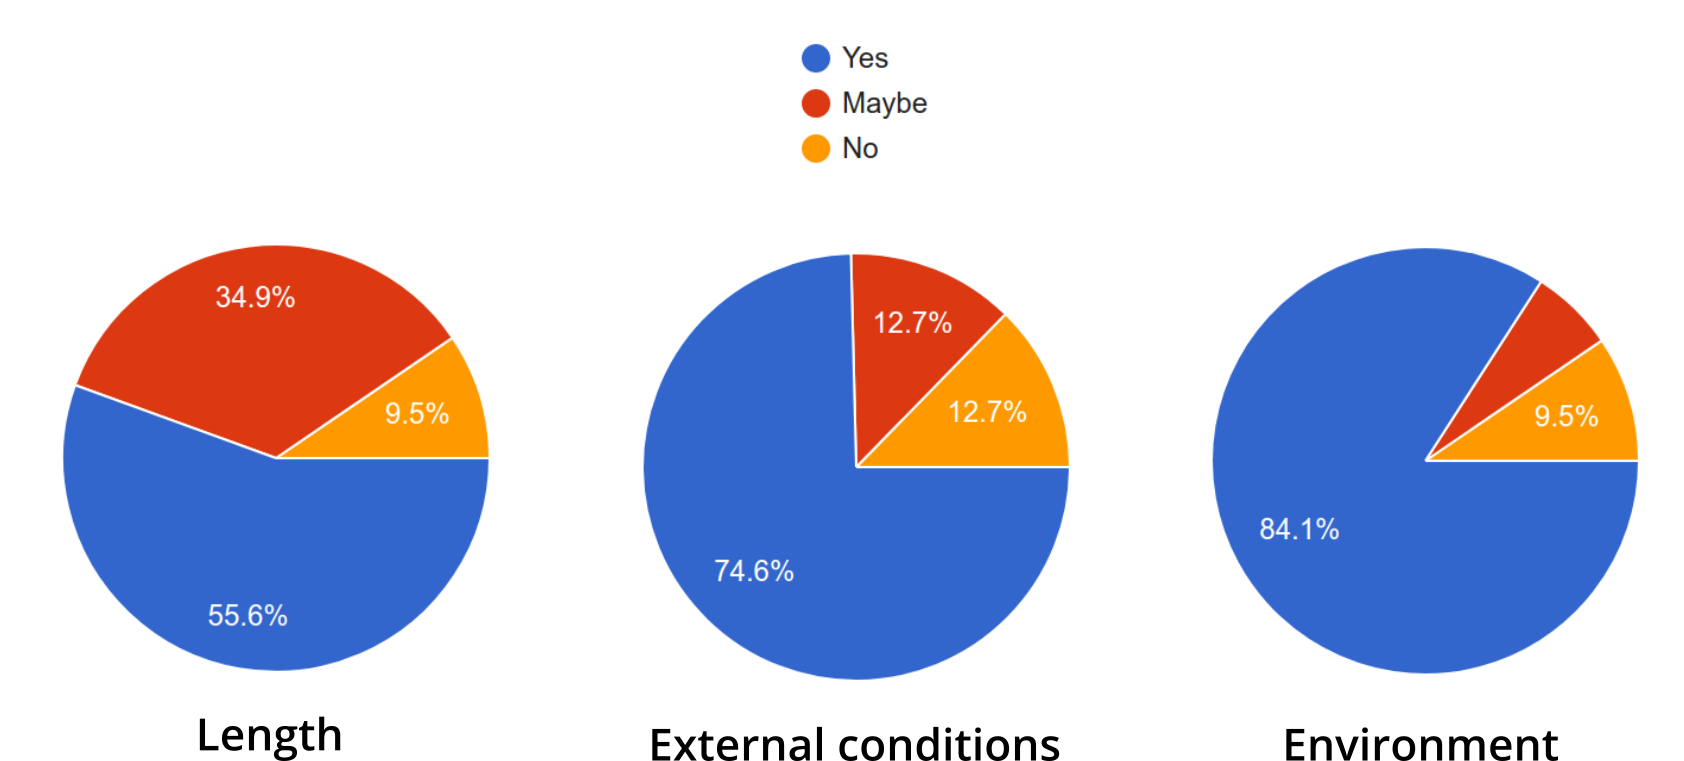
\includegraphics[width=0.9\linewidth]{0-graph_influences.png}
  \end{center}
  \caption{Sleep detection comparison between consumer devices}
  \label{fig:influence}
\end{figure}

As to what sleep means to them, they were asked how much on scale of 1 to 10 does the sleep quality corelate with their daily performance. Performance was separated in 3 different categories - task performance, mood and physical performance. Task performance is described as perceived efficiency of work and school task completion quality and speed. Mood is also quite important aspect as good mood may effect both professional and private life. Influence of sleep on physical performance may be quite important for students involved in competitive sports activities and a good quality sleep may help them improve their performance. Average, median and standard deviation of these results are displayed in \ref{tab:influence}.

\begin{table}[h]
  \begin{center}
    \begin{tabular}[h]{ | >{\centering\arraybackslash} m{4cm} | >{\centering\arraybackslash} m{2cm} | >{\centering\arraybackslash} m{2cm} | >
    {\centering\arraybackslash} m{2cm} |  }
      \hline
      Influence & Average & Standard deviation & Median \\ 
      \hline
      \\[-1em]
      Daily task performance & 7.51 & 1.42 & 8 \\ 
      \\[-1em]
      Mood & 7.54 & 1.49 & 8 \\
      \\[-1em]
      Physical performance & 7.40 & 1.28 & 8 \\
      \hline
    \end{tabular}
  \end{center}
  \caption{Perceived influence of sleep on scale of 1 to 10.}
  \label{tab:influence}
\end{table}

Little more than a half (57\%) of participants are familiar with sleep tracking devices but only 27\% have used a non obtrusive sleep tracking device. Out of all poll participants, 6 have tested their quality of sleep using clinical methods such as \ac{EEG}, \ac{EMG} or \ac{EOG}. As widely available sleep trackers are still quite new to the market, 76.5\% of the participants owning a sleep tracking device have been in a possession of it for less then a year. More than a half (58.7\%) of participants that own a sleep tracking device indicate that they check their sleep quality on a weekly basis or more frequently while 29.4\% people are checking their devices rarely. A relative majority of 41.2\% indicates that data received from the device didn't make them change their sleep habits while 35.3\% indicate that they have changed their sleep routines. The rest of 23.5\% participants are not certain. Most of the poll participants indicated that for sleep tracking they use smartbands with the cheapest one (Xiaomi Mi Band) being the most popular. But a considerable amount of 29.4\% participants have also used their smartphones for sleep tracking. These are not precise devices and methods and only 5.9\% of group says that they wouldn't like to have a more precise and detailed device to track their sleep. 

\begin{figure}[h]
  \begin{center}
    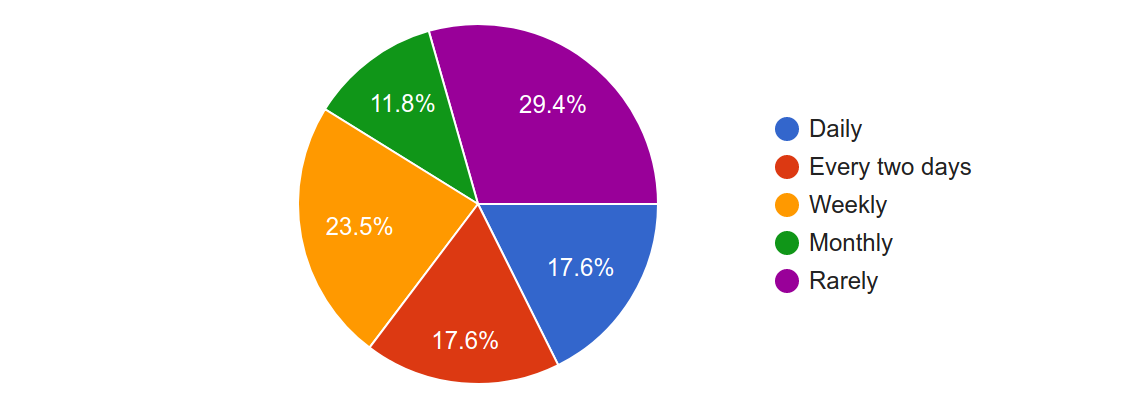
\includegraphics[width=0.8\linewidth]{0-graph_check.png}
  \end{center}
  \caption{Frequency of sleep data review by poll participants}
  \label{fig:check}
\end{figure}

So what can be concluded from this poll? Well, there is a large market share of younger adults who are not familiar with sleep tracking devices. Even if they are familiar, most of them don't own one despite perceiving that data obtained from those devices could help them sleep better. This means that market for sleep tracking devices has a very large potential growth.


\section{Goal and scope}

This thesis will try to describe a novel implementation which will track sleep for both clinical and consumer purposes improving on the quality of tracking and simplicity of use over the currently available solutions. Proposed solution is based on a pressure sensor mesh network which is placed under the mattress and which tracks the movement and vital signs of the sleepers. It continues on the previous work done at \ac{UC-Lab} at \ac{HTWG} and enhances it by providing system architecture, hardware and software required to achieve a goal of precise contactless sleep tracking. Thesis also proposes an interface that can be used to collect and analyse acquired data and will serve as a stepping stone for the future research.

Hardware is designed in such a way that it allows an easy installation and so that all of the components are widely available and easily replaceable. Thesis describes design decisions in detail with the proposal of future improvements in terms of features, reliability and precision. Embedded software setup is based on open-source solutions which are not tied to a specific platform which means that an end product may use the same software albeit possible changes in hardware. Application software provides user interface for analysis of data but also provides an \ac{API} which allows other services to access the data in a standardized way. Together the whole system will allow recording, tracking and analysis of sleep data and will be tested in a suitable environment.

In this scope, reader will be acquainted with the process of design and implementation of such a system. Problems regarding communication between sensor nodes, endpoint data collection and graphical data display will be described in detail. Thesis will also present and give an insight into the results of how system functions. Possibilities for implementation of preprocessing, filtering and automatic sleep analysis will also be presented. What will not be in focus of this thesis however are the medical aspects of sleep recognition and sleep stage classification. They will be considered and reviewed, as they are critical to the functional aspect of the project, but they remain to be described and analysed in a future research to which this thesis will hopefully serve as a technological foundation.


\section{Thesis outline}

Before the new system design is proposed a current one found at \ac{UC-Lab} will be presented and reviewed. Current system design decisions will be shown along with the implementation based details in \autoref{chap:evolution}. Focus in \autoref{chap:nodes} will be on implementation of a mesh network nodes that will serve the purpose of data collection from the sensors. It will present design considerations and decisions that led to the final product. Details on an embedded system serving as and endpoint will be described in the \autoref{chap:endpoint}. In it a part of application software which takes care of communication between the endpoint and sensor nodes will also be described. In \autoref{chap:display} it will be shown how data is stored and displayed and how it can be used by other services. Measurement results will be shown in the \autoref{chap:results} after which a conclusion will be drawn in \autoref{chap:conclusion}.